% GNUPLOT: LaTeX picture with Postscript
\begingroup
  \makeatletter
  \providecommand\color[2][]{%
    \GenericError{(gnuplot) \space\space\space\@spaces}{%
      Package color not loaded in conjunction with
      terminal option `colourtext'%
    }{See the gnuplot documentation for explanation.%
    }{Either use 'blacktext' in gnuplot or load the package
      color.sty in LaTeX.}%
    \renewcommand\color[2][]{}%
  }%
  \providecommand\includegraphics[2][]{%
    \GenericError{(gnuplot) \space\space\space\@spaces}{%
      Package graphicx or graphics not loaded%
    }{See the gnuplot documentation for explanation.%
    }{The gnuplot epslatex terminal needs graphicx.sty or graphics.sty.}%
    \renewcommand\includegraphics[2][]{}%
  }%
  \providecommand\rotatebox[2]{#2}%
  \@ifundefined{ifGPcolor}{%
    \newif\ifGPcolor
    \GPcolorfalse
  }{}%
  \@ifundefined{ifGPblacktext}{%
    \newif\ifGPblacktext
    \GPblacktexttrue
  }{}%
  % define a \g@addto@macro without @ in the name:
  \let\gplgaddtomacro\g@addto@macro
  % define empty templates for all commands taking text:
  \gdef\gplfronttext{}%
  \gdef\gplfronttext{}%
  \makeatother
  \ifGPblacktext
    % no textcolor at all
    \def\colorrgb#1{}%
    \def\colorgray#1{}%
  \else
    % gray or color?
    \ifGPcolor
      \def\colorrgb#1{\color[rgb]{#1}}%
      \def\colorgray#1{\color[gray]{#1}}%
      \expandafter\def\csname LTw\endcsname{\color{white}}%
      \expandafter\def\csname LTb\endcsname{\color{black}}%
      \expandafter\def\csname LTa\endcsname{\color{black}}%
      \expandafter\def\csname LT0\endcsname{\color[rgb]{1,0,0}}%
      \expandafter\def\csname LT1\endcsname{\color[rgb]{0,1,0}}%
      \expandafter\def\csname LT2\endcsname{\color[rgb]{0,0,1}}%
      \expandafter\def\csname LT3\endcsname{\color[rgb]{1,0,1}}%
      \expandafter\def\csname LT4\endcsname{\color[rgb]{0,1,1}}%
      \expandafter\def\csname LT5\endcsname{\color[rgb]{1,1,0}}%
      \expandafter\def\csname LT6\endcsname{\color[rgb]{0,0,0}}%
      \expandafter\def\csname LT7\endcsname{\color[rgb]{1,0.3,0}}%
      \expandafter\def\csname LT8\endcsname{\color[rgb]{0.5,0.5,0.5}}%
    \else
      % gray
      \def\colorrgb#1{\color{black}}%
      \def\colorgray#1{\color[gray]{#1}}%
      \expandafter\def\csname LTw\endcsname{\color{white}}%
      \expandafter\def\csname LTb\endcsname{\color{black}}%
      \expandafter\def\csname LTa\endcsname{\color{black}}%
      \expandafter\def\csname LT0\endcsname{\color{black}}%
      \expandafter\def\csname LT1\endcsname{\color{black}}%
      \expandafter\def\csname LT2\endcsname{\color{black}}%
      \expandafter\def\csname LT3\endcsname{\color{black}}%
      \expandafter\def\csname LT4\endcsname{\color{black}}%
      \expandafter\def\csname LT5\endcsname{\color{black}}%
      \expandafter\def\csname LT6\endcsname{\color{black}}%
      \expandafter\def\csname LT7\endcsname{\color{black}}%
      \expandafter\def\csname LT8\endcsname{\color{black}}%
    \fi
  \fi
  \setlength{\unitlength}{0.0400bp}%
  \begin{picture}(4000.00,4000.00)%
    \gplgaddtomacro\gplfronttext{%
      \colorrgb{0.00,0.00,0.00}%
      \put(388,793){\makebox(0,0)[r]{\strut{}\footnotesize $0$}}%
      \colorrgb{0.00,0.00,0.00}%
      \put(388,1158){\makebox(0,0)[r]{\strut{}\footnotesize $2$}}%
      \colorrgb{0.00,0.00,0.00}%
      \put(388,1522){\makebox(0,0)[r]{\strut{}\footnotesize $4$}}%
      \colorrgb{0.00,0.00,0.00}%
      \put(388,1887){\makebox(0,0)[r]{\strut{}\footnotesize $6$}}%
      \colorrgb{0.00,0.00,0.00}%
      \put(388,2251){\makebox(0,0)[r]{\strut{}\footnotesize $8$}}%
      \colorrgb{0.00,0.00,0.00}%
      \put(388,2616){\makebox(0,0)[r]{\strut{}\footnotesize $10$}}%
      \colorrgb{0.00,0.00,0.00}%
      \put(388,2980){\makebox(0,0)[r]{\strut{}\footnotesize $12$}}%
      \colorrgb{0.00,0.00,0.00}%
      \put(388,3345){\makebox(0,0)[r]{\strut{}\footnotesize $14$}}%
      \colorrgb{0.00,0.00,0.00}%
      \put(520,573){\makebox(0,0){\strut{}\footnotesize $6$}}%
      \colorrgb{0.00,0.00,0.00}%
      \put(885,573){\makebox(0,0){\strut{}\footnotesize $8$}}%
      \colorrgb{0.00,0.00,0.00}%
      \put(1249,573){\makebox(0,0){\strut{}\footnotesize $10$}}%
      \colorrgb{0.00,0.00,0.00}%
      \put(1614,573){\makebox(0,0){\strut{}\footnotesize $12$}}%
      \colorrgb{0.00,0.00,0.00}%
      \put(1978,573){\makebox(0,0){\strut{}\footnotesize $14$}}%
      \colorrgb{0.00,0.00,0.00}%
      \put(2343,573){\makebox(0,0){\strut{}\footnotesize $16$}}%
      \colorrgb{0.00,0.00,0.00}%
      \put(2708,573){\makebox(0,0){\strut{}\footnotesize $18$}}%
      \colorrgb{0.00,0.00,0.00}%
      \put(3072,573){\makebox(0,0){\strut{}\footnotesize $20$}}%
      \colorrgb{0.00,0.00,0.00}%
      \put(3437,573){\makebox(0,0){\strut{}\footnotesize $22$}}%
      \colorrgb{0.00,0.00,0.00}%
      \put(-118,2069){\rotatebox{90}{\makebox(0,0){\strut{}$y$ [m]}}}%
      \colorrgb{0.00,0.00,0.00}%
      \put(2069,243){\makebox(0,0){\strut{}$x$ [m]}}%
    }%
    \gplgaddtomacro\gplfronttext{%
    }%
    \put(0,0){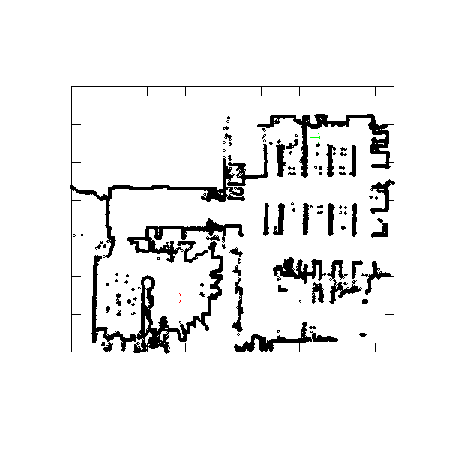
\includegraphics[scale=0.8]{./figures/slides/ch3/csal}}%
    \gplfronttext
  \end{picture}%
\endgroup
